\chapter{Introduction}

Linear Algebra is a branch of Mathematics. Many applied problems from
Science, Engineering and Finance can be written in terms of Linear
Algebra questions. This is also true of Calculus, which is why these
two fields are stressed in undergraduate Mathematics education at UBC
and other universities. By putting a class of commonly occurring
problems into a unified, abstract framework, the problems can be
studied in detail and well understood. This understanding can then be
taken back to problems in many different fields. It is especially
important to realize that very large problems (with potentially
millions of unknowns) can be understood in the same framework as the
model problems we do by hand in these courses. This course has
computer labs that involve the mathematical software, MATLAB, that
will allow you to solve larger problems using numerical computations. 

Unlike Calculus, Linear Algebra does not require a lot of background
knowledge. Basic operations in Linear Algebra are just
arithmetic. However, there is a powerful connection between these
simple arithmetic operations and geometric quantities. Simple ideas in
this course start to become abstract when combined together. Linear
Algebra is a subject you can study with very limited matematical 
background, but
you are advised to keep up with course lectures, readings, assignments
and computer labs so you won't be left behind at the transition from
concrete ideas to abstract ones.

\section{Course Goals}

The goal of the course is to enable students to 
\begin{enumerate}
\item recognize linear algebra questions (for which there are
straight-forward analytic and numerical solution techniques) as parts
of applied problems
\item make the connection between geometric properties and analytic
quantities (determinants, dot and cross products, eigenvalues, etc.)
\item recognize that linear systems of equations can have unique,
infinite or no solutions and know how to determine all solutions or
that none exist
\item recognize matrix multiplication as a linear transformation and
that such transformations (to the same dimensional space) can be
simplified using eigen-analysis
\item use complex numbers, which arise naturally in the eigen-analysis
of matrices
\end{enumerate}

\section{About the Subject} 

The subject of the course is Linear Algebra, focussing on four main
topics: 
\begin{enumerate}
\item vectors and matrices and connections to geometry
\item linear systems
\item complex numbers 
\item eigen-analysis of matrices
\end{enumerate} 
Several applications are considered. The two applications that come up repeatedly in the notes are resistor networks and random walks. 

\subsection{Connection to Geometry}

The first topic considered in the course is vectors, which are
quantities with both magnitude and direction. A typical quantity
represented as a vector is a force $\bf F$ on an object as shown in
Figure~\ref{fig_intro1}. The force $\bf F$ in that figure acts in the
$x-y$ plane as shown. The vector force $\bf F$ can be represented by
its components $(F_x, F_y)$. Some interesting questions you will be
able to answer after completing this course are: what directions are
perpendicular to this force?; what are the coordinates of the force in
the rotated coordinate system $x^\prime - y^\prime$?; what are the
coordinates of the force if its direction is rotated? These last two
questions are related.
\begin{figure}
\centerline{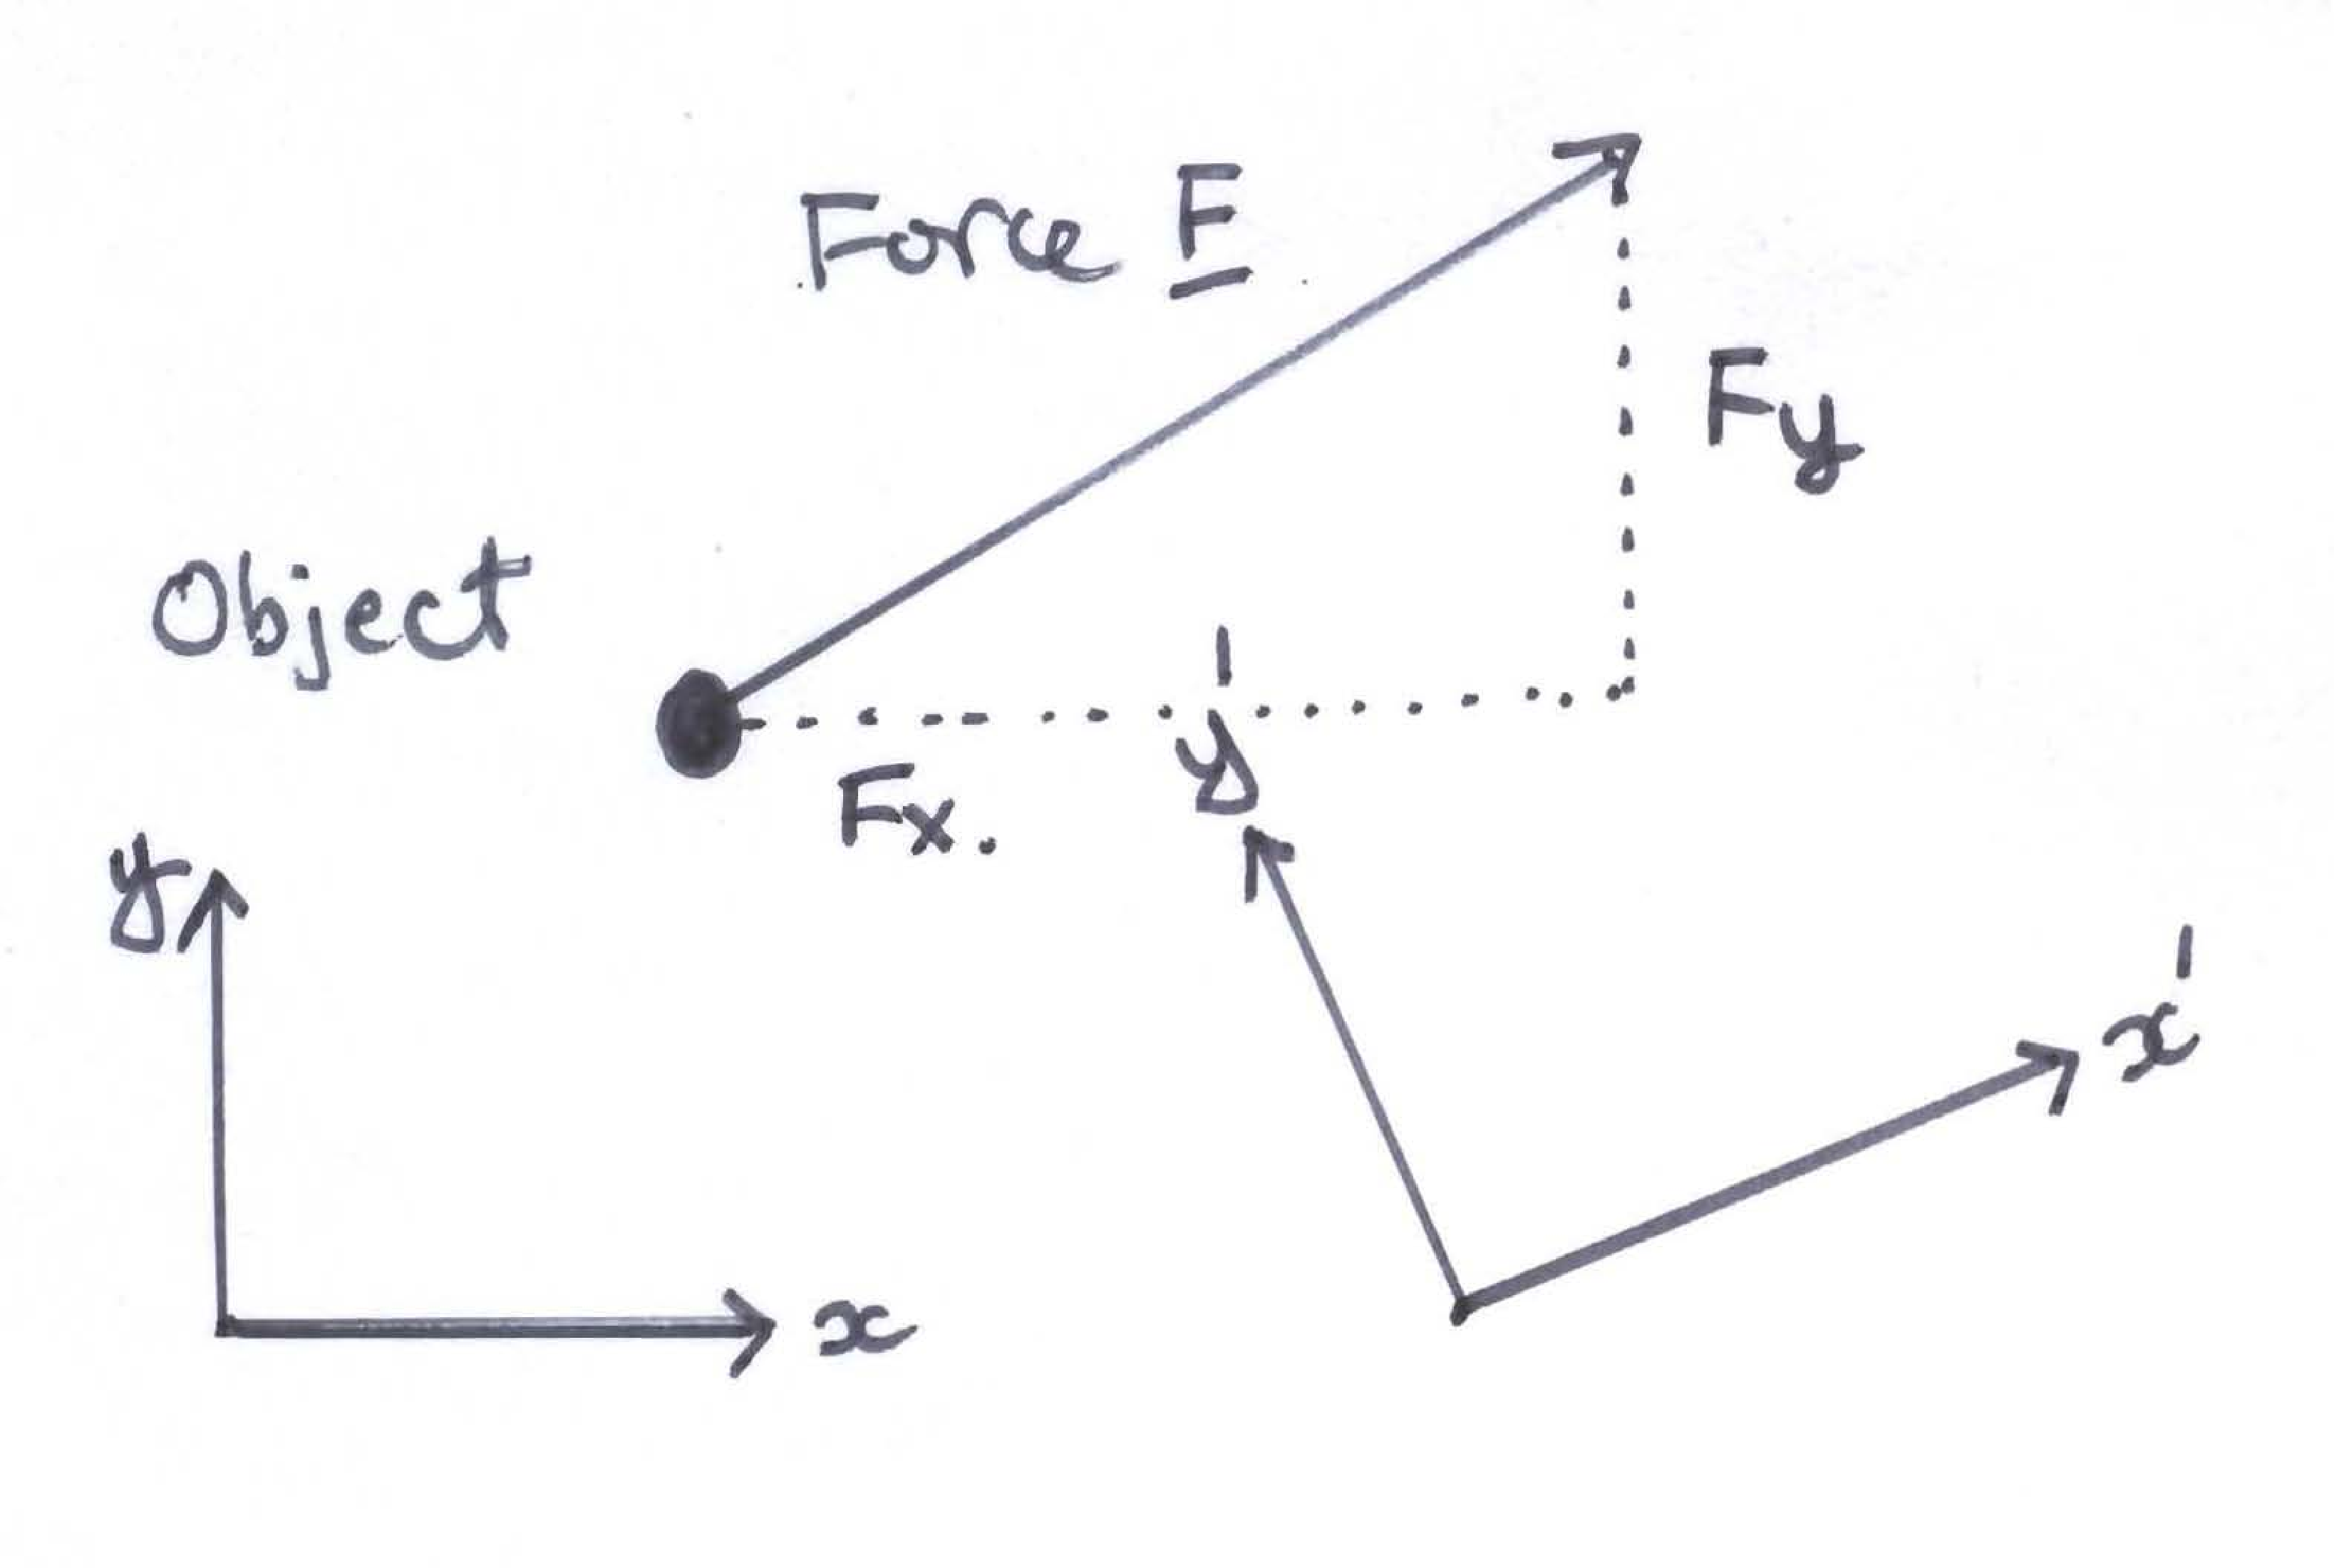
\includegraphics[height=4cm]{1_introfig1}}
\caption{\label{fig_intro1} Force vector and coordinate systems.}
\end{figure}

\subsection{Linear Systems}

Consider the following simple example. You probably saw something like
this in high school. 

\begin{example} Bob and Sue together have 12 dollars. Sue has
2 dollars more than Bob. How much money do each have? 
{\rm You can probably guess the solution by trial and error, but let us
proceed a bit more formally. Let $x$ be the amount of money Sue has
and $y$ the amount Bob has. The two statements in the example can be
written mathematically as
\begin{eqnarray*}
x + y & = & 12 \\
x - y & = & 2.
\end{eqnarray*}
The equations above are a {\em linear system} for the unknowns $x$ and
$y$. A technique that can be used to solve the system (that is,
determine the values of $x$ and $y$ that {\em simultaneously} solve
both equations above) is substitution. The second equation can be
written as
\[
x = y+2
\]
This can be substituted into the first equation above, {\em
eliminating} $y$ from the problem
\[
(y+2) + y = 12 \mbox{\   or $2y +2 = 12$ \ so $2y = 10$ \ so $y=5$}
\]
The value of $y=5$ determines $x=7$ from either of the original
relationships. Thus it is determined that Bob has 5 dollars and Sue
has 7. }
\end{example}

Often (but not always) a linear system of $n$ equations for $n$
unknowns has a unique solution. The example above was for the case
$n=2$. However, the substitution technique used above becomes
impractical when $n$ is larger than 3. In this course you will learn
the Gaussian Elimination technique to solve linear systems. This
systematic method can find all solutions when there are any and also
determine if the system has no solutions. This method can be
implemented in numerical software and used to solve very large
systems.

\subsection{Eigen-analysis} 

The final subject of the course is eigen-analysis of matrices and its
applications. A simple, motivational example comes from the study of
discrete dynamical systems. Consider a sequence of values 
\[
x_0, x_1, \cdots x_n \cdots
\]
where the index $n$ is a time level. Suppose that $x_n$ is determined
by the previous value $x_{n-1}$ in the same way for every $n$, that is
\begin{equation}
\label{eq:intro1}
x_n = f(x_{n-1}) \mbox{\ \ for every $n \geq1 $} 
\end{equation}
for a given function $f$. This could describe the population number $x_n$
of a species at year $n$. The simple model assumes that the population 
the next year only depends on the population this year through the 
function $f$. 
If the initial value $x_0$ were given, then
the values $x_1, x_2 \cdots x_n \cdots$ could be determined using
(\ref{eq:intro1}) repeatedly. A linear problem arises when we take the
specific example $f(x) = ax$ where $a$ is a given constant. In this
case, it is easy to compute the entries of the sequence:
\begin{eqnarray*}
x_1 & = & f(x_0) = a x_0 \\ 
x_2 & = & f(x_1) = f(a x_0) = a^2 x_0 \\ 
\vdots & & \vdots \\
x_n & = & f(x_{n-1})) = a^n x_0
\end{eqnarray*}
For this example, we can determine how the sequence behaves very well
because we have an expression for $x_n$ above that is easy to
understand. There are several cases:
\begin{enumerate}
\item If $x_0 = 0$ then $x_n =0$ for all $n$. 
\item if $|a|< 1$ then $\lim_{n \rightarrow \infty} x_n = 0$.
\item if $a=1$ then $x_n = x_0$ for all $n$.
\item if $a=-1$ then the values alternate in sign: $x_n$ has the value
$x_0$ is $n$ is even, $-x_0$ if $n$ is odd.
\item if $|a|>1$ and $x_0 \neq 0$ then the values of the sequence grow
in absolute value as $n \rightarrow \infty$.
\end{enumerate}

Linear discrete dynamical systems for vectors are also of interest. In
these cases, multiplication by the number $a$ in the example above is
replaced by multiplication by a matrix $\bf A$. Eigen-analysis of the
matrix $\bf A$ allows one to understand how the system behaves as $n
\rightarrow \infty$ in a similar way to the simple example above. Eigen-analysis naturally involves complex arithmetic, so this is introduced in the notes beforehand. 

\section{About The Computer Labs}

The course includes six one-hour computer labs. These are given to
small groups of students every other week starting in the {\em second}
week of the term. It is a good idea
to read through the lab notes before going to the lab so you are ready
to begin in the lab. After your first lab, you will be able to go to
the lab rooms in open hours to improve your MATLAB skills and to
prepare for upcoming labs. Computer lab material including your knowledge
of MATLAB commands will be tested on midterms and the final exam. 

There are two main goals for the labs. The first is to gain
familiarity with the computational tool, MATLAB, that is commonly used
in later courses and Engineering careers. The second is to be able to
solve larger, more interesting applied problems that would otherwise
be inaccessible using analytic methods. Seeing the algorithms of
MATLAB in action may also help you understand the underlying
mathematical concepts you see in the lectures.

\section{About These Notes}

\begin{description}
\item[2004:] 
The first version of these notes was written by Richard Froese for
Math 152 taught in the Spring of 2004. There are many text books on
elementary linear algebra material, but none have the material in the
order we want for Math 152 for Applied Science students. These notes
stress geometric concepts in two and three dimensional space. They
also treat applications and numerical approximation using MATLAB in
more detail than most texts. For this reason, the authors have felt it
was worthwhile to maintain and improve these notes for Math
152. Additionally, we believe it is a social benefit for students to
have access to this material without having to purchase an expensive,
commercial text.
\item[2007:] 
An update to the notes was made by Richard Froese for the course in
2007, including solutions to the exercises. 
\item[2009:] The version written for
the 2009 course had some updates by Brian Wetton: this introductory
chapter, some additional comments on MATLAB commands, a reworked
section on linear systems arising from electrical networks, and
additional problems and solutions. In addition, the notes were 
converted to standard \LaTeX format to make them easier to maintain. 
\item[2010:] 
Substantial revisions for the notes for 2010 were done by Ignacio Rozada, who was supported 
by a UBC Skylight grant over the Summer of 2009 to add the problems 
and solutions used in weekly assignments the previous year. He also 
added additional MATLAB material. Brian Wetton added additional notes 
to Chapter 4 on the use of matrix multiplication and inverses in the 
derivation of solutions to the ``fundamental problem" of resistor 
networks.
\item[2015:] Brian Wetton added many additional examples to Chapter 2 and added more formal 
definitions of the key concepts: linear combination, span, linear independence, basis and dimension. He also added material in Chapter 5 on the use of complex arithmetic in complex linear systems and determinants. 
Joel Feldman contributed an additional topics section to Chapter 3 on the checksum technique. 
Hand drawn resistor network diagrams were replaced throughout the text by Egor Dontsov. The material on 
complex numbers was split off into a separate chapter.
\item[2017:] Brian Wetton corrected errors in the notes pointed out by the 2016 class and added a discussion in the first section of Chapter 4 on the interpretation of matrix vector multiplication as a linear combination of the columns of the matrix.
\item[2025:] Colin B. Macdonald started tracking changes in a Git repo,
posted these notes to GitHub, and fixed some typos.
\end{description} 
Further revisions are planned. There will be additional MATLAB
material added to the notes and additional problems and solutions. The Chapter on complex numbers needs some revision.
If you have any suggestions for additional
material or ways to improve the presentation, please contact the maintainers
at
{\tt https://github.com/UBCMath/Math152notes}


% \end{document}
